\documentclass[tikz,border=1pt]{standalone} 
\usepackage{tikz}
\usepackage{pgfplots}
\begin{document}
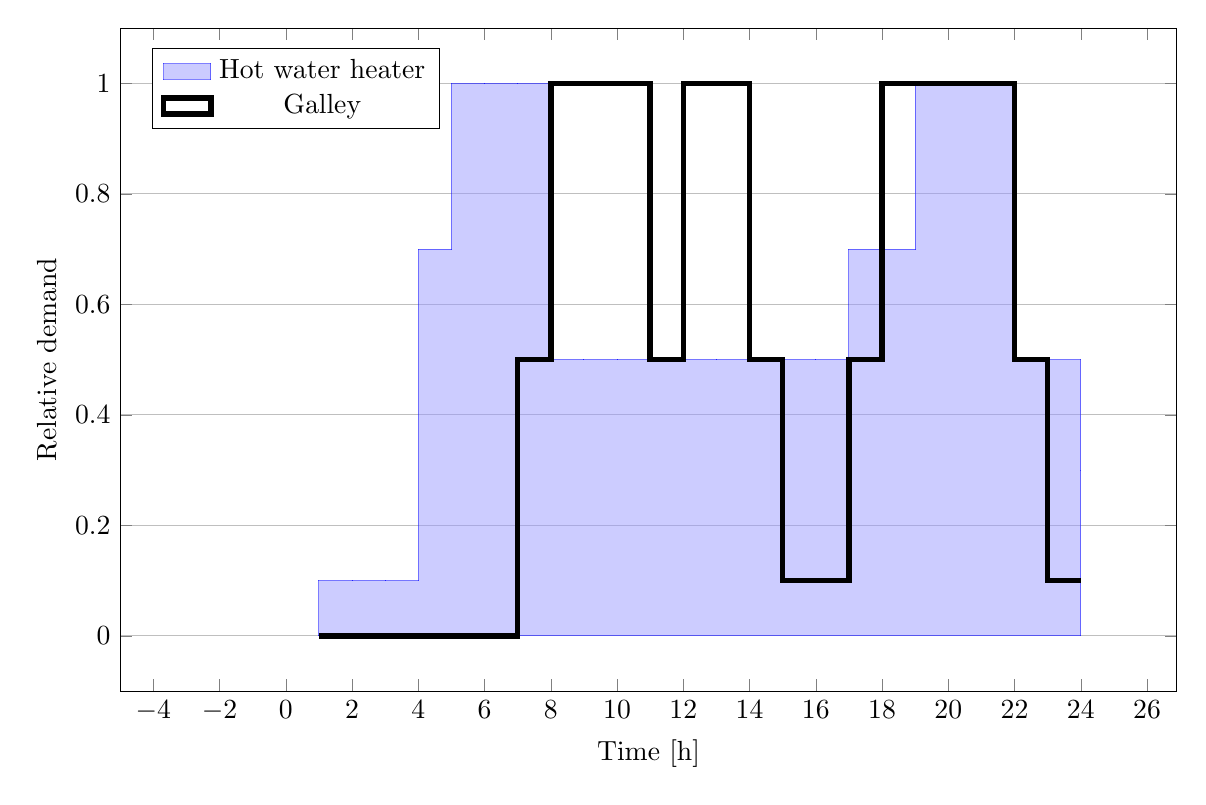
\begin{tikzpicture}
\begin{axis}[
	xlabel={Time [h]},
	ylabel={Relative demand},
	height=10cm, width=15cm,
	ymajorgrids,
	area legend,
	legend pos = north west,
	xmin=-5,
]
\addplot+[const plot, mark=none, fill=blue!40!white, opacity=0.5, line width=0]
coordinates
{(1,0.1)  (2,0.1)   (3,0.1)
 (4,0.7) (5,1.0)  (6,1.0)  (7,1.0)
 (8,0.5) (9,0.5)  (10,0.5) (11,0.5)
(12,0.5)	(13,0.5)	(14,0.5)	(15,0.5)	(16,0.5)
(17,0.7)	(18,0.7)	(19,1.0)	(20,1.0)	(21,1.0)
(22,0.5)	(23,0.5)	(24,0.3)} \closedcycle;
\addlegendentry{Hot water heater}

\addplot+[const plot, mark=none, color=black, line width=2pt]
coordinates
{(1,0.0)  (2,0.0)   (3,0.0)
	(4,0.0) (5,0.0)  (6,0.0)  (7,0.5)
	(8,1.0) (9,1.0)  (10,1.0) (11,0.5)
	(12,1.0)	(13,1.0)	(14,0.5)	(15,0.1)	(16,0.1)
	(17,0.5)	(18,1.0)	(19,1.0)	(20,1.0)	(21,1.0)
	(22,0.5)	(23,0.1)	(24,0.1)};
\addlegendentry{Galley}
\end{axis}

\end{tikzpicture}
\end{document}